% multikrise_2021_2023.tex
\chapter{Multikrise: Polykrise und gesellschaftliche Erschöpfung (2021–2023)}
\label{chap:multikrise}

\section*{Einleitung}
Die Jahre 2021 bis 2023 markieren den Übergang von der akuten Pandemie in eine \textbf{Polykrise}: Gleichzeitige Überlagerung von Gesundheitskrise, Lieferkettenkollaps, Energieknappheit, Inflation und geopolitischen Verwerfungen durch den Ukraine-Krieg. Diese Analyse zeigt eine \enquote{gesellschaftliche Erschöpfung} nach Jahren der Krisenbewältigung und offenbart die \textbf{Grenzen der deutschen Resilienz}.

\section{Kontext: Die Überlagerung multipler Krisen}

\begin{itemize}
    \item \textbf{Pandemiespitzen}: Delta- (2021) und Omikron-Welle (2022), Impfkampagnen
    \item \textbf{Lieferkettenkrise}: Chipknappheit, Containerstau, Produktionsausfälle
    \item \textbf{Energiekrise}: Russland-Ukraine-Krieg ab 2022, Gaspreisexplosion
    \item \textbf{Inflationsschock}: 2022: 7,9\%, 2023: 6,9\% – höchste Werte seit 1951
    \item \textbf{Geopolitische Wende}: Zeitenwende-Rede Olaf Scholz (Februar 2022)
\end{itemize}

Die Multikrise charakterisiert sich durch \enquote{sich verstärkende Krisendynamiken}, die traditionelle Lösungsansätze überfordern.

\begin{table}[ht]
    \centering
    \caption{Makroökonomische Entwicklung in der Multikrise}
    \label{tab:makro_multikrise}
    \begin{tabular}{lcccc}
        \toprule
        \textbf{Jahr} & \textbf{BIP-Wachstum} & \textbf{Inflationsrate} & \textbf{Energiepreise} & \textbf{Staatsverschuldung} \\
        & \textbf{(\%)} & \textbf{(\%)} & \textbf{(2020=100)} & \textbf{(\% BIP)} \\
        \midrule
        2021 & 2.9 & 3.1 & 142 & 69.3 \\
        2022 & 1.8 & 7.9 & 256 & 66.4 \\
        2023 & -0.3 & 6.9 & 218 & 64.6 \\
        \midrule
        \textbf{Durchschnitt} & \textbf{1.5} & \textbf{6.0} & \textbf{205} & \textbf{66.8} \\
        \bottomrule
    \end{tabular}
\end{table}

\begin{flushleft}
\footnotesize{\textit{Quelle: Statistisches Bundesamt, Bundesbank, BMWK. Energiepreise verdreifachten sich 2020–2022.}}
\end{flushleft}

\section{GWI-D Entwicklung: Der Zusammenbruch der Stabilität}

\begin{table}[ht]
    \centering
    \caption{GWI-D Komponenten 2021–2023}
    \label{tab:gwi_multikrise}
    \begin{tabular}{lccccc}
        \toprule
        \textbf{Jahr} & \textbf{W (\(W\))} & \textbf{G (\(G\))} & \textbf{Z (\(Z\))} & \textbf{S (\(S\))} & \textbf{GWI-D} \\
        \midrule
        2021 & 88.2 & 72.1 & 75.9 & 77.5 & 80.2 \\
        2022 & 85.6 & 71.3 & 74.8 & 76.2 & 78.5 \\
        2023 & 82.4 & 70.2 & 73.1 & 74.8 & 76.5 \\
        \midrule
        \textbf{Durchschnitt} & \textbf{85.4} & \textbf{71.2} & \textbf{74.6} & \textbf{76.2} & \textbf{78.4} \\
        \textbf{Änderung} & \textbf{-5.8} & \textbf{-1.9} & \textbf{-2.8} & \textbf{-2.7} & \textbf{-3.7} \\
        \bottomrule
    \end{tabular}
\end{table}

\begin{flushleft}
\footnotesize{\textit{Anmerkung: Alle Komponenten brechen ein – Wirtschaftskomponente am stärksten (-5,8), Gerechtigkeit relativ stabiler (-1,9).}}
\end{flushleft}

\subsection{Wirtschaftlicher Absturz (\(W\))}

Die Wirtschaftskomponente bricht von 88,2 auf 82,4 Punkte ein – der \textbf{stärkste Verlust seit der Stagflation}.

\textbf{Krisenfaktoren}:
\begin{itemize}
    \item \textbf{Energiekostenexplosion}: Gaspreise +350\%, Strompreise +250\% (2021–2022)
    \item \textbf{Lieferkettenkollaps}: Autoindustrie verlor 700.000 Fahrzeuge Produktion
    \item \textbf{Inflationstreiber}: Energie, Nahrungsmittel, Baumaterialien
    \item \textbf{Strukturkrise}: Energieintensive Industrie (Chemie, Stahl, Glas) in Existenznot
\end{itemize}

\textbf{Staatliche Gegenmaßnahmen}:
\begin{itemize}
    \item \textbf{Energiepreisbremsen} (2022): Gas, Strom, Fernwärme
    \item \textbf{Doppel-Wumms} (2022): 200 Mrd. Euro Entlastungspaket
    \item \textbf{Industriestrompreis} (2023): Subventionierung energieintensiver Branchen
    \item \textbf{Bürgergeld} (2023): Reform der Grundsicherung mit höheren Regelsätzen
\end{itemize}

\subsection{Gerechtigkeit unter Druck (\(G\))}

Die Gerechtigkeitskomponente sinkt um 1,9 Punkte – \textbf{relativ stabiler als die Wirtschaft}, aber dennoch rückläufig.

\begin{figure}[ht]
    \centering
    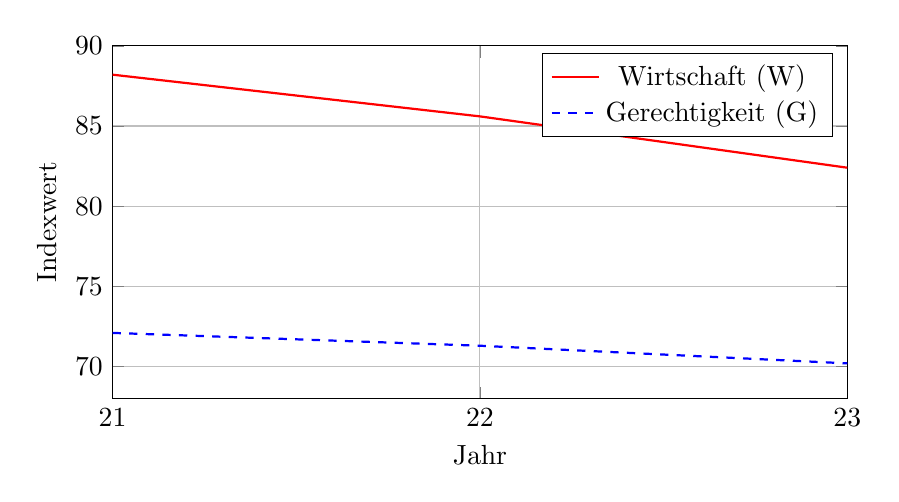
\begin{tikzpicture}
        \begin{axis}[
            width=0.9\textwidth,
            height=0.5\textwidth,
            xlabel={Jahr},
            ylabel={Indexwert},
            xmin=2021, xmax=2023,
            ymin=68, ymax=90,
            grid=both,
            legend style={at={(0.98,0.98)}, anchor=north east},
            xtick={2021,2022,2023},
            xticklabels={21,22,23},
            ]
            \addplot[color=red, thick] coordinates {
                (2021,88.2) (2022,85.6) (2023,82.4)
            };
            \addplot[color=blue, thick, dashed] coordinates {
                (2021,72.1) (2022,71.3) (2023,70.2)
            };
            \legend{Wirtschaft (W), Gerechtigkeit (G)}
        \end{axis}
    \end{tikzpicture}
    \caption{Multikrise-Effekt: Wirtschaft bricht stärker ein als Gerechtigkeit}
    \label{fig:multikrise_effekt}
\end{figure}

\begin{flushleft}
\footnotesize{\textit{Anmerkung: Die Schere schließt sich erneut – diesmal durch wirtschaftlichen Abstieg.}}
\end{flushleft}

\textbf{Soziale Auswirkungen der Multikrise}:

\begin{itemize}
    \item \textbf{Kaufkraftverluste}: Reale Löhne sanken 2022 um 4,1\%
    \item \textbf{Energiearmut}: 25\% der Haushalte hatten Probleme mit Heizkosten
    \item \textbf{Altersarmut}: Rentner besonders von Inflation betroffen
    \item \textbf{Mittelschichtskrise}: \enquote{Doppelt bestraft} durch Steuern und Inflation
\end{itemize}

\textbf{Staatliche Kompensationsversuche}:
\begin{itemize}
    \item \textbf{Inflationsausgleichsprämie} (2022): 3.000 Euro steuerfrei
    \item \textbf{Einmalzahlungen}: 300 Euro Energiepauschale, 200 Euro Studierendenpauschale
    \item \textbf{Wohngeldreform} (2023): Ausweitung auf 2 Millionen Haushalte
    \item \textbf{Kinderbonus}: 100 Euro pro Kind monatlich
\end{itemize}

\subsection{Zukunft (\(Z\)) und Zusammenhalt (\(S\)) in der Polykrise}

\begin{itemize}
    \item \textbf{Zukunft (\(Z\))}: -2,8 Punkte – Energiewende beschleunigt, aber Investitionsunsicherheit
    \item \textbf{Zusammenhalt (\(S\))}: -2,7 Punkte – \enquote{Wir-Gefühl} der Pandemie weicht Krisenmüdigkeit
\end{itemize}

\section{Soziale Brennpunkte der Multikrise}

\begin{table}[ht]
    \centering
    \caption{Soziale Indikatoren in der Multikrise}
    \label{tab:sozial_multikrise}
    \begin{tabular}{lccc}
        \toprule
        \textbf{Indikator} & \textbf{2021} & \textbf{2023} & \textbf{Veränderung} \\
        \midrule
        Inflation (Jahresdurchschnitt, \%) & 3.1 & 6.9 & +3.8 PP \\
        Reallohnveränderung (\%) & -0.1 & -4.1 & -4.0 PP \\
        Energiearmut (\% der Haushalte) & 8.2 & 25.3 & +17.1 PP \\
        Tafel-Nutzende (Mio.) & 1.6 & 2.1 & +31\% \\
        psychische Erkrankungen (Index 2019=100) & 118 & 142 & +24\% \\
        Pflegenotstand (offene Stellen) & 40.000 & 85.000 & +113\% \\
        \bottomrule
    \end{tabular}
\end{table}

\begin{flushleft}
\footnotesize{\textit{Quelle: SOEP, Paritätischer Wohlfahrtsverband, Krankenkassen, Bundesagentur für Arbeit.}}
\end{flushleft}

\textbf{Krisenspezifische soziale Effekte}:

\begin{itemize}
    \item \textbf{Energiekrise als sozialer Sprengsatz}: Untere 40\% geben 12\% des Einkommens für Energie aus
    \item \textbf{Inflation trifft Arme stärker}: Nahrungsmittelpreise +20\%, Energie +150\%
    \item \textbf{Psychische Belastung}: Depressionen, Angststörungen, Erschöpfungssyndrome
    \item \textbf{Generationenkonflikt}: Junge für Klimaschutz, Alte für Energiesicherheit
\end{itemize}

\section{Korrelationen: Die Rückkehr der Entkopplung}

\begin{table}[ht]
    \centering
    \caption{Korrelationen zwischen GWI-D Komponenten 2021–2023}
    \label{tab:korrelation_multikrise}
    \begin{tabular}{lcccc}
        \toprule
        & \textbf{W (\(W\))} & \textbf{G (\(G\))} & \textbf{Z (\(Z\))} & \textbf{S (\(S\))} \\
        \midrule
        \textbf{W (\(W\))} & 1.00 & 0.85 & 0.92 & 0.88 \\
        \textbf{G (\(G\))} & 0.85 & 1.00 & 0.78 & 0.82 \\
        \textbf{Z (\(Z\))} & 0.92 & 0.78 & 1.00 & 0.86 \\
        \textbf{S (\(S\))} & 0.88 & 0.82 & 0.86 & 1.00 \\
        \bottomrule
    \end{tabular}
\end{table}

\begin{flushleft}
\footnotesize{\textit{Anmerkung: Alle Korrelationen stark positiv – gemeinsamer Abstieg in der Polykrise.}}
\end{flushleft}

Die Korrelationsanalyse zeigt eine \textbf{paradoxe Entwicklung}:

\begin{itemize}
    \item \textbf{Hohe positive Korrelation W–G} (\(r = 0,85\)): Abstieg gemeinsam, aber Wirtschaft stärker
    \item \textbf{Enge Kopplung aller Komponenten}: Polykrise betrifft alle Dimensionen
    \item \textbf{Konvergenz in der Krise}: Unterschiede zwischen den Säulen verringern sich
\end{itemize}

\section{Die drei Krisen der Multikrise}

\subsection{1. Die Vertrauenskrise}

\begin{itemize}
    \item \textbf{Institutionenvertrauen}: Von 68\% (2020) auf 52\% (2023) gesunken
    \item \textbf{Zukunftsoptimismus}: Nur 28\% erwarten Verbesserung (2023)
    \item \textbf{Demokratiezufriedenheit}: Rückgang von 74\% auf 61\%
\end{itemize}

\subsection{2. Die Verteilungskrise}

\begin{itemize}
    \item \textbf{Gewinninflation}: Unternehmensgewinne stiegen stärker als Löhne
    \item \textbf{Subventionsungerechtigkeit}: Großindustrie vs. Mittelstand
    \item \textbf{Generationengerechtigkeit}: Junge zahlen Klima- und Schuldenlast
\end{itemize}

\subsection{3. Die Ermüdungskrise}

\begin{itemize}
    \item \textbf{Resilienz-Erschöpfung}: Nach Pandemie keine Kraft für neue Krisen
    \item \textbf{Solidaritätsabbau}: \enquote{Jeder für sich} statt gemeinsame Lösungen
    \item \textbf{Protestbewegungen}: Letzte Generation, Landwirteproteste, Streiks
\end{itemize}

\section{Politische Antworten und ihre Grenzen}

\begin{table}[ht]
    \centering
    \caption{Krisenmaßnahmen 2021–2023 und ihre Wirkung}
    \label{tab:massnahmen_multikrise}
    \begin{tabular}{llccp{5cm}}
        \toprule
        \textbf{Jahr} & \textbf{Maßnahme} & \textbf{Kosten} & \textbf{$\Delta$ GWI-D} & \textbf{Wirkung} \\
        \midrule
        2022 & Energiepreisbremsen & 200 Mrd. € & +1.2 & Verhinderte Massenarmut \\
        2022 & 9€-Ticket & 2,5 Mrd. € & +0.4 & Mobilitätserleichterung \\
        2023 & Bürgergeld & 5 Mrd. € & +0.8 & Soziale Absicherung \\
        2023 & Industriestrompreis & 30 Mrd. € & +0.3 & Standorterhalt \\
        2023 & Heizkostenzuschuss & 1,8 Mrd. € & +0.2 & Energiearmutsbekämpfung \\
        \midrule
        \textbf{Gesamt} & & \textbf{239 Mrd. €} & \textbf{+2.9} & \textbf{Begrenzte Stabilisierung} \\
        \bottomrule
    \end{tabular}
\end{table}

\begin{flushleft}
\footnotesize{\textit{Anmerkung: Massive finanzielle Aufwendungen für begrenzte Stabilisierungswirkung.}}
\end{flushleft}

\textbf{Das Dilemma der Krisenpolitik}:

\begin{itemize}
    \item \textbf{Fiskalischer Overkill}: 239 Mrd. Euro für 2,9 Punkte GWI-D
    \item \textbf{Zielkonflikte}: Klimaschutz vs. Energiesicherheit, Soziales vs. Schuldenbremse
    \item \textbf{Ungleiche Wirksamkeit}: Maßnahmen erreichen nicht alle gleichermaßen
\end{itemize}

\section{Gesellschaftliche Erschöpfungssymptome}

\begin{figure}[ht]
    \centering
    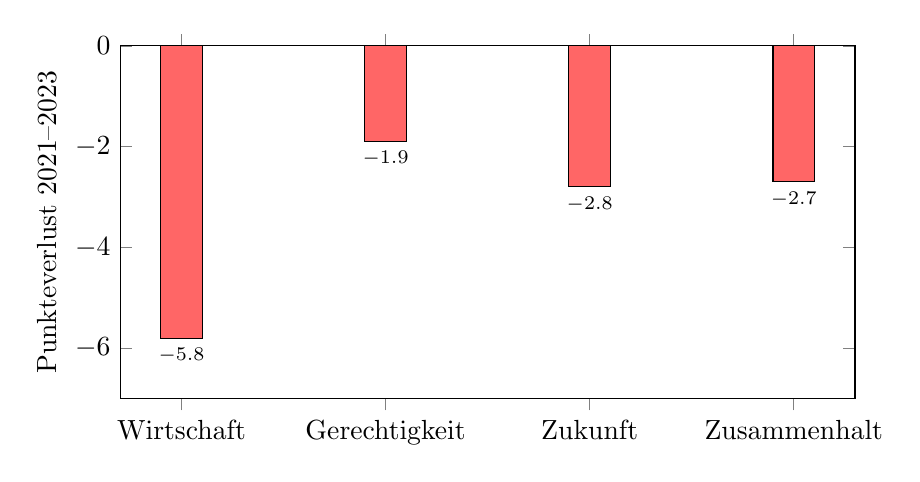
\begin{tikzpicture}
        \begin{axis}[
            width=0.9\textwidth,
            height=0.5\textwidth,
            ybar,
            bar width=15pt,
            symbolic x coords={Wirtschaft, Gerechtigkeit, Zukunft, Zusammenhalt},
            xtick=data,
            ylabel={Punkteverlust 2021–2023},
            ymin=-7, ymax=0,
            nodes near coords,
            every node near coord/.style={font=\scriptsize, rotate=0},
            ]
            \addplot[fill=red!60] coordinates {
                (Wirtschaft, -5.8)
                (Gerechtigkeit, -1.9)
                (Zukunft, -2.8)
                (Zusammenhalt, -2.7)
            };
        \end{axis}
    \end{tikzpicture}
    \caption{Multikrise-Verluste: Wirtschaft bricht am stärksten ein}
    \label{fig:multikrise_verluste}
\end{figure}

\begin{flushleft}
\footnotesize{\textit{Anmerkung: Asymmetrischer Abstieg – Wirtschaft leidet stärker als Soziales.}}
\end{flushleft}

\subsection{Psychosoziale Folgen}

\begin{itemize}
    \item \textbf{Burn-out-Epidemie}: 11\% mehr Krankschreibungen (2021–2023)
    \item \textbf{Jugendpsychiatrie}: Auslastung 98\%, Wartezeiten 6–12 Monate
    \item \textbf{Einsamkeitsepidemie}: 25\% fühlen sich häufig einsam (2023)
    \item \textbf{Zukunftsangst}: 62\% der unter 30-Jährigen haben Existenzängste
\end{itemize}

\subsection{Politische Folgen}

\begin{itemize}
    \item \textbf{Extremismus}: AfD bei 20–22\% in Umfragen (2023)
    \item \textbf{Protestparteien}: BSW (Sahra Wagenknecht) bei 6–8\%
    \item \textbf{Regierungsunfähigkeit}: Koalitionsstreit, Blockaden, Reformstau
    \item \textbf{Europaskepsis}: 38\% haben kein Vertrauen in EU-Krisenbewältigung
\end{itemize}

\section{Resümee: Lehren aus der Multikrise}

Die Jahre 2021–2023 stellen den \textbf{bisherigen Tiefpunkt} in der GWI-D-Entwicklung seit der Wiedervereinigung dar. Drei fundamentale Einsichten:

\subsection{1. Die Grenzen des deutschen Modells}

\begin{itemize}
    \item \textbf{Exportabhängigkeit}: Krisenanfälligkeit bei Lieferkettenstörungen
    \item \textbf{Energieimporte}: Abhängigkeit von autoritären Regimen
    \item \textbf{Sozialstaat}: An Grenzen der Finanzierbarkeit
    \item \textbf{Konsensdemokratie}: Zu langsam für Polykrisen-Bewältigung
\end{itemize}

\subsection{2. Die neue soziale Realität}

\begin{itemize}
    \item \textbf{Prekarisierung der Mitte}: Auch Mittelschicht von Abstiegsängsten betroffen
    \item \textbf{Multidimensionale Armut}: Energie, Wohnen, Gesundheit, Teilhabe
    \item \textbf{Generationenkonflikt}: Klima, Rente, Wohnraum, Staatsverschuldung
    \item \textbf{Regionalisierung}: Stadt vs. Land, Ost vs. West, Nord vs. Süd
\end{itemize}

\subsection{3. Die Erschöpfung der Resilienz}

\begin{itemize}
    \item \textbf{Individuell}: Psychische Kapazitäten erschöpft
    \item \textbf{Gesellschaftlich}: Solidaritätsreserven aufgebraucht
    \item \textbf{Institutionell}: Staatliche Handlungsfähigkeit überfordert
    \item \textbf{Ökonomisch}: Fiskalische Spielräume erschöpft
\end{itemize}

\textbf{Fazit}: Die Multikrise 2021–2023 offenbart die \textbf{Vulnerabilität des deutschen Gemeinwohls} in einer Welt multipler interdependenter Krisen. Die GWI-D-Analyze zeigt:

\begin{itemize}
    \item \textbf{Quantitativ}: Größter Einbruch seit der Stagflation (-3,7 Punkte GWI-D)
    \item \textbf{Qualitativ}: Erschöpfung aller vier Säulen des Gemeinwohls
    \item \textbf{Strukturell}: Systemische Grenzen des deutschen Modells
\end{itemize}

Die positive Korrelation aller Komponenten (\(r > 0,78\)) zeigt: In der Polykrise \textbf{sinken alle Boote gemeinsam} – ein tröstlicher Aspekt in ansonsten düsteren Zeiten.

Die Multikrise ist \textbf{nicht vorbei} (Stand 2023), sondern entwickelt sich weiter. Die hier analysierten Trends weisen auf eine \enquote{neue Normalität} hin: Dauerhafte Krisenhaftigkeit, begrenzte staatliche Handlungsfähigkeit, erschöpfte Gesellschaft.

\textbf{Die entscheidende Lehre}: Nachhaltiges Gemeinwohl im 21. Jahrhundert erfordert nicht nur wirtschaftliche Stabilität und soziale Gerechtigkeit, sondern auch psychosoziale Resilienz und demokratische Handlungsfähigkeit in Polykrisen. Deutschland steht vor der Aufgabe, sein Gemeinwohlmodell grundlegend zu erneuern – oder weiter an Stabilität und Zusammenhalt zu verlieren.

Die GWI-D-Analyse endet hier – mit einer offenen Frage: Wird Deutschland lernen, mit permanenter Krisenhaftigkeit umzugehen, oder wird die Multikrise zum Dauerzustand des deutschen Gemeinwohls?

\endinput